\documentclass[12pt]{article}

\input{C:/Users/ilden/Documents/School/TeX памятка/header.tex}

\begin{document}
	\tableofcontents
	\setcounter{tocdepth}{3}
	\newpage
	\section{Механика.}
	\begin{definition}
		Механическое движение~--- изменение пространственного положения тела относительно других тел с течением времени.
	\end{definition}
	\begin{definition}
		При поступательном движении прямая проведенная через любые две точки внутри тела остается параллельна сама себе.
	\end{definition}
	\begin{definition}
		При вращательном движении каждая точка тела вращается по своей окружности, центры этих окружностей лежат на одной прямой, прямая называется осью вращения.
	\end{definition}
	\begin{statement}
		Любое движение~--- сумма этих двух движений.
	\end{statement}
	\begin{definition}
		Колебательное движение~--- движение, повторяющееся с той или иной точностью во времени.
	\end{definition}
	\subsection{Кинематика.}
	\begin{definition}
		Кинематика~--- раздел механики, изучающий способы описания движения и связь величин характеризующих это движение.
	\end{definition}
	\begin{statement}
		Для описания движения нужны:
		\begin{itemize}
			\item Система отсчета.
			\item Тело отсчета.
			\item Система координат.
			\item Часы.
		\end{itemize}
	\end{statement}
	\begin{statement}
		Способы анализа:
		\begin{itemize}
			\item Табличный.
			\item Графический.
			\item Аналитический.
		\end{itemize}
	\end{statement}
	\subsubsection{Равномерное прямолинейное движение.}
	\begin{definition}
		Равномерное прямолинейное движение~--- за любые равные промежутки времени тело проходит одинаковые участки пути, траектория при этом прямая линия.
	\end{definition}
	\begin{definition}
		Траектория~--- кривая, по которой движется тело.
	\end{definition}
	\begin{definition}
		Путь~--- длинна траектории.
	\end{definition}
	\begin{definition}
		Перемещение~--- вектор из начальной точки в конечную.
	\end{definition}
	\begin{definition}
		Расстояние~--- модуль перемещения.
	\end{definition}
	\begin{definition}
		Скорость~--- физическая векторная величина, характеризующая быстроту изменения положения тела в пространстве. $V = \frac{S}{t}$.
	\end{definition}
	\noindent
	\textbf{Формулы.} \\
	\begin{tabular}{|c|c|c|}
		\hline
		\textbf{Величина} & \textbf{РПД} & \textbf{РУД} \\
		\hline
		 & & \\
		Скорость & $V = \frac{S}{t}$ & $V_x = V_{0x} + at$ \\
		 & & \\
		\hline
		 & & \\
		Расстояние & $S = V \cdot t$ & $S = V_{0x}t + \frac{at^2}{2}$ \\
		 & & \\
		\hline
		 & & \\
		Координата & $x = x_0 + V_{0x}t$ & $x = x_0 + V_{0x}t + \frac{at^2}{2}$ \\
		 & & \\
		\hline
	\end{tabular}
	\begin{statement}[Золотая формула механики.]
		$S = \frac{V_{\text{к}}^2 - V_0^2}{2a}$.
	\end{statement}
	\subsubsection{Движение под углом горизонта.}
	Тело брошено с высоты $h$ под углом $\alpha$ со скоростью $V_0$.
	\begin{enumerate}
		\item $V_x = V_0 \cos\alpha$
		\item $x = V_0 \cos\alpha t$
		\item $V_y = V_0 \sin\alpha - gt$
		\item $y = h_0 + V_0 \sin\alpha t - \frac{gt^2}{2}$
	\end{enumerate}
	I. Траектория.
	\begin{quote}
		$t = \frac{x}{V_0 \cos\alpha}$. \\
		$y = h_0 + V_0 \sin\alpha \frac{x}{V_0 \cos\alpha} - \frac{g}{2} \cdot \frac{x^2}{V_0^2 \cos^2\alpha}$. \\
		$y = h_0 + x \tg\alpha - \frac{gx^2}{2V_0^2\cos^2\alpha}$. \\
	\end{quote}
	II. $H_{max}$: $V_{y} = 0$.
	\begin{quote}
		$0 = V_0 \sin\alpha - gt_{\text{падения}}$. \\
		$t_{\text{падения}} = \frac{V_0 \sin\alpha}{g}$. \\
		$H_{max} = h_0 + V_0 \sin\alpha \cdot \frac{V_0 \sin\alpha}{g} - \frac{g}{2} \cdot \frac{V_0^2 \sin^2\alpha}{g^2}$. \\
		$H_{max} = h_0 + \frac{V_0^2 \sin^2\alpha}{2g}$. \\
	\end{quote}
	III. $t_{\text{полета}}$: $y = 0$.
	\begin{quote}
		$0 = h_0 + V_0 \sin\alpha t_{\text{полета}} - \frac{gt_{\text{полета}}^2}{2}$. \\
		$\frac{gt_{\text{полета}}^2}{2} - V_0 \sin\alpha t_{\text{полета}} - h_0 = 0$. \\
		$t_{\text{полета}} = \frac{V_0 \sin\alpha + \sqrt{V_0^2\sin^2\alpha + 2gh_0}}{g}$. \\
	\end{quote}
	IV. Дальность полета: $L$.
	\begin{quote}
		$L = x(t_{\text{полета}}) = V_0 \cos\alpha t_{\text{полета}}$. \\
		$L = \frac{V_0^2 \sin2\alpha}{g}$. \\
	\end{quote}
	V. Конечная скорость.
	\begin{quote}
		$V_{\text{y к}} = V_0 \sin\alpha - gt_{\text{полета}} = V_0 \sin\alpha - g \cdot \frac{V_0 \sin\alpha}{g} - g \cdot \frac{\sqrt{V_0^2 \sin^2\alpha + 2gh_0}}{g}$. \\
		$V_{\text{x к}} = V_0 \cos\alpha$. \\
		$V_{\text{y к}} = -\sqrt{V_0^2 \sin^2\alpha + 2gh_0}$. \\
		$V_{\text{к}} = \sqrt{V_{\text{x к}}^2 + V_{\text{y к}}^2} = \sqrt{V_0^2 \cos^2\alpha + V_0^2 \sin^2\alpha + 2gh_0}$. \\
		$V_{\text{к}} = \sqrt{V_0^2 + 2gh_0}$. \\
	\end{quote}
	VI. Угол падения ($\beta$).
	\begin{quote}
		$\cos\beta = \frac{V_x}{V_{\text{к}}} = \frac{V_0 \cos\alpha}{\sqrt{2gh_0 + V_0^2}}$.
	\end{quote}
	\subsubsection{Векторный подход к задачам с броском под углом горизонта (баллистическим задачам).}
	Тело брошено под углом $\alpha$ со скоростью $V_0$. \\
	$\vec{V} = \vec{V_0} + gt$. \\
	$\vec{r} = \vec{V_0} + \frac{\vec{g}t^2}{2}$.
	\begin{figure}[H]
		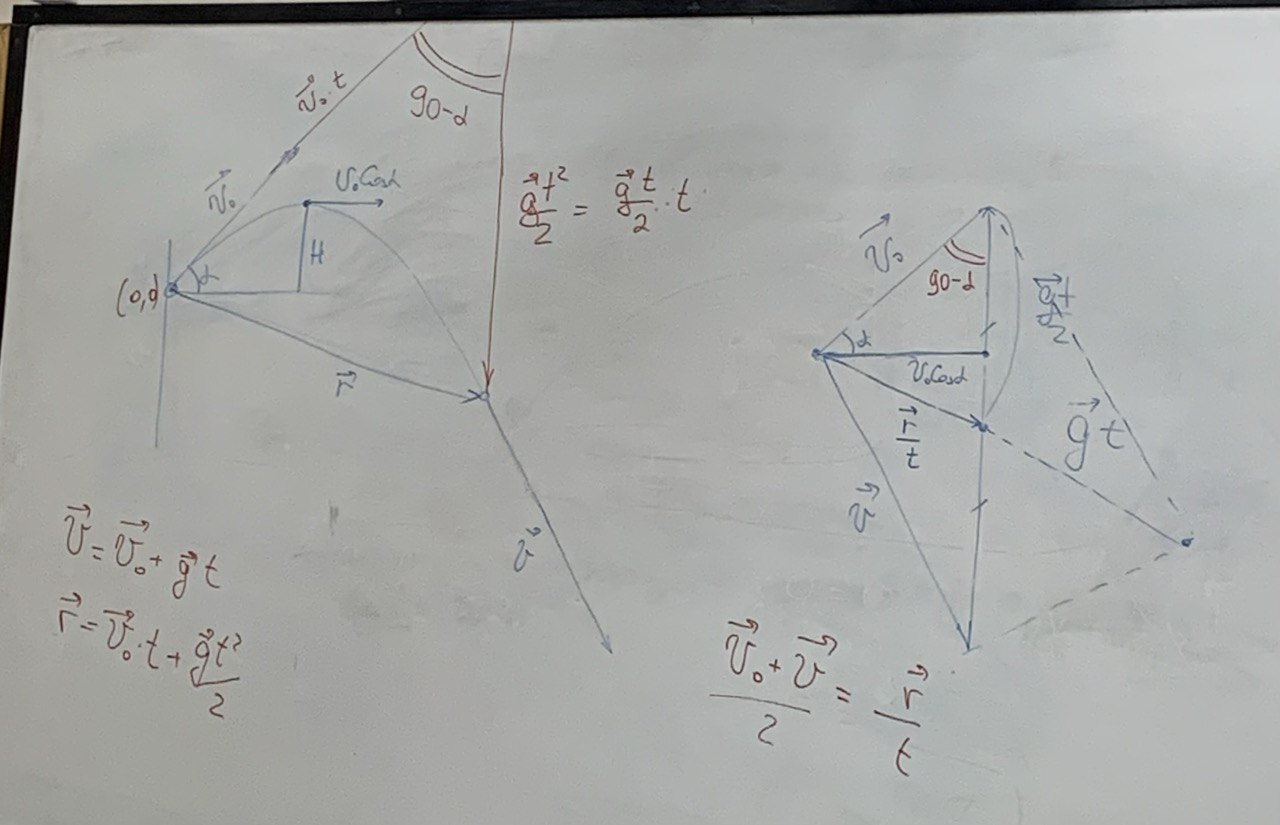
\includegraphics[height=200px]{extra-materials/Скорости_Вектора_1}
		\caption{Треугольник скоростей и путей.}
	\end{figure}
	$S_{\triangle V} = \frac{V_0 \cdot \cos\alpha \cdot gt}{2} = \frac{V \cdot V_0 \cdot \sin(\alpha + \beta)}{2}$.
	\begin{figure}[H]
		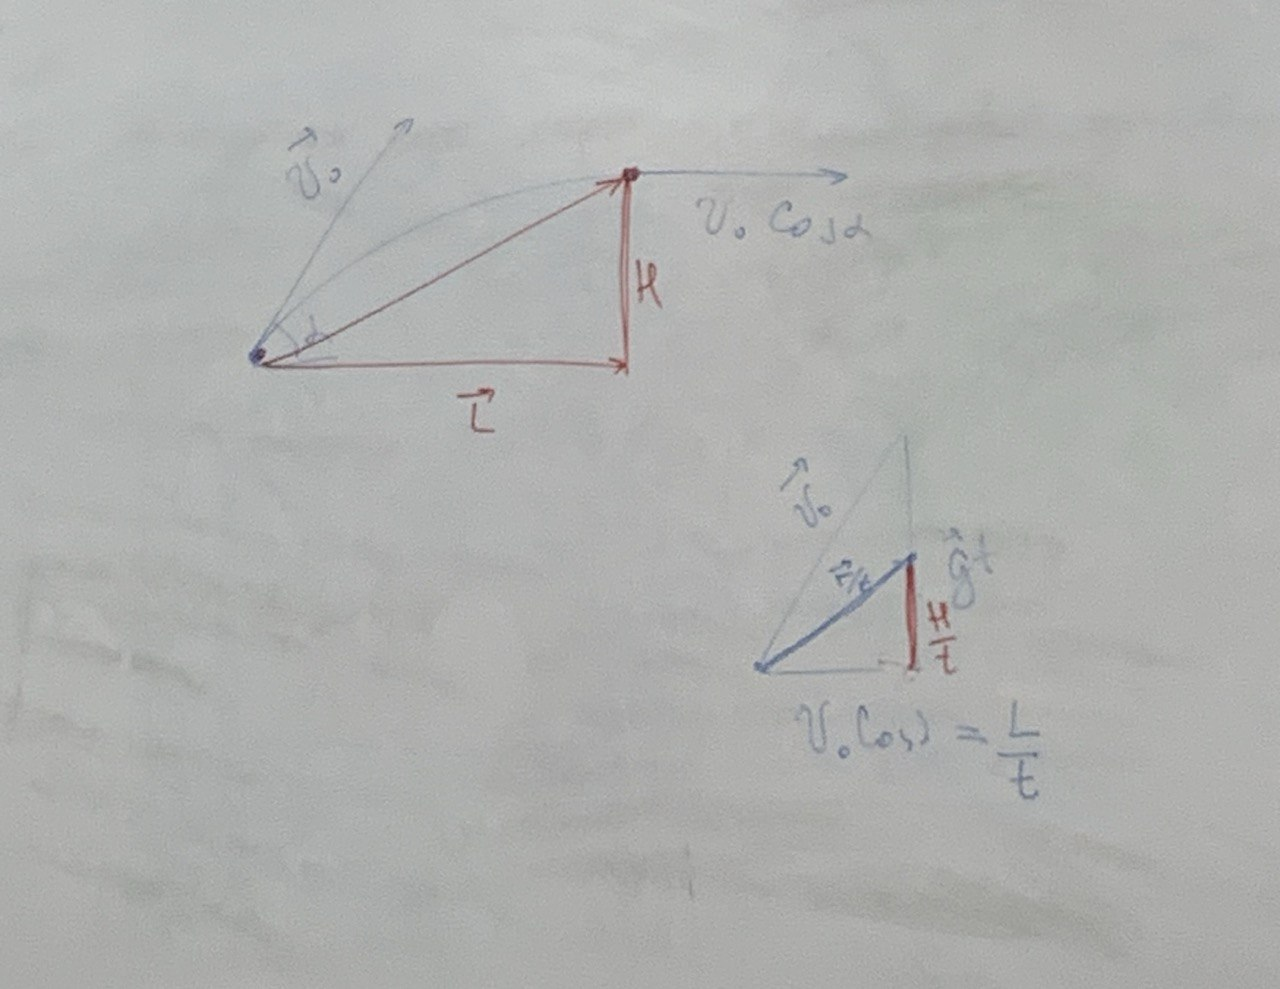
\includegraphics[height=200px]{extra-materials/Скорости_Вектора_2}
		\caption{Треугольник скоростей 2.}
	\end{figure}
	\subsubsection{Движение по окружности.}
	\begin{figure}[H]
		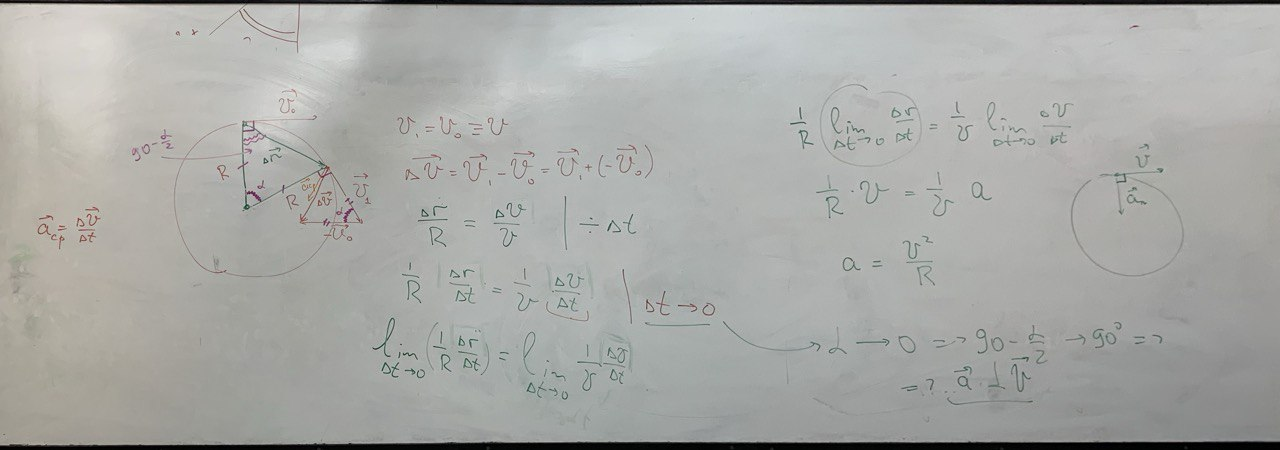
\includegraphics[height=120px]{extra-materials/Скорости_Вектора_3}
		\caption{Движение по окружности.}
	\end{figure}
	\begin{definition}
		$\omega$ --- угловая скорость. $\omega = \lim_{\varDelta t \rightarrow 0} \frac{\varDelta \varphi}{\varDelta t}$.
	\end{definition}
	\begin{definition}
		Период~--- время, за которое тело проходит полный оборот по окружности. $T = \frac{2\pi R}{V} = \frac{2\pi}{\omega}$.
	\end{definition}
	\begin{statement}[Формула связи линейной скорости с угловой.]
		$V = \omega R$.
	\end{statement}
	\begin{definition}
		Частота~--- количество оборотов в секунду. $\nu = \frac{1}{T}$. $[\nu] = $ Гц.
	\end{definition}
	\noindent
	$\beta = \lim_{\varDelta t \rightarrow 0} \frac{\varDelta \omega}{\varDelta t} = const$. \\
	$\beta = \frac{\varDelta \omega}{\varDelta t} = \frac{\omega(t) - \omega_0}{t - t_0}$. \\
	$\omega(t) = \omega_0 + \beta t$. \\
	$\varphi = \varphi_0 \pm \omega_0t \pm \frac{\beta t^2}{2}$. \\
	$a_{\tau} = \beta R$.
	\subsubsection{Относительность движение. Преобразование Галилея.}
	\begin{definition}
		Принцип относительности классической механики~--- во всех инерциальных системах отсчета механические явления протекают одинаково.
	\end{definition}
	\noindent
	$\vec{V_{\text{абс}}} = \vec{V_{\text{относ}}} + \vec{V_{\text{пер}}}$
	\subsection{Динамика.}
	\begin{definition}
		Динамика~--- отвечает на вопрос, почему тело движется именно так.
	\end{definition}
	\noindent
	$\vec{F}$, $[F] = \text{Н}$.
	\begin{definition}
		Инерция~--- способность тела сохранять скорость при отсутствие внешнего воздействия.
	\end{definition}
	\begin{definition}
		Три закона Ньютона:
		\begin{enumerate}[1.]
			\item Существуют инерциальные системы отсчета (ИСО). ИСО --- те системы отсчета, в которых если на тело не действуют силы или их действие скомпенсировано, то тело движется равномерно и прямолинейно или покоится.
			\item $\sum\vec{F} = m\vec{a}$. \\
			Инертность --- свойство тела, которое заключается в том, что для изменения скорости тела необходимо время.
			\item При взаимодействие двух тел возникает две силы. Эти две силы приложены к двум разным телам, равным по модулю, противоположны по направлению, лежат на одной прямой, имеют одну природу (гравитационная, электромагнитная, сильная, слабая).
		\end{enumerate}
	\end{definition}
	\begin{statement}[Ограничения на законы]
		Работают только для скоростей много меньших скоростей света, в инерциальных системах счисления и с ненулевыми массами.
	\end{statement}
	\begin{statement}
		Полезная информация:
		\begin{enumerate}
			\item Тело стоит на платформе, платформа движется вверх с ускорением $\vec{a}$, у тела масса $m$, то $P = m \cdot (g + a)$.
			\item Тело стоит на платформе, платформа движется вниз с ускорением $\vec{a}$, у тела масса $m$, то $P = m \cdot (g - a)$.
		\end{enumerate}
	\end{statement}
	\subsubsection{Сила трения.}
	\begin{definition}
		Сила трения имеет электро-магнитную природу. Направленна вдоль поверхности противодействующих поверхностей, против относительной скорости взаимодействия двух тел.
	\end{definition}
	\begin{definition}
		$F_{\text{тр}} = N\mu$; $\mu$~--- коэффициент трения.
	\end{definition}
	\begin{statement}
		Не существует силы вязкого трения покоя.
	\end{statement}
	\subsubsection{Сила упругости.}
	\begin{definition}
		Сила упругости~--- сила электромагнитной природы, возникающая при деформации, направленная против деформации. $F_{\text{упр}} = -k \varDelta x$.
	\end{definition}
	\begin{definition}
		Виды деформаций:
		\begin{itemize}
			\item Упругие (обратимая деформация):
			\begin{enumerate}
				\item Растяжение-сжатие
				\item Сдвиг
				\item Изгиб
				\item Кручение
			\end{enumerate}
			\item Пластическая (необратимая деформация).
		\end{itemize}
	\end{definition}
	\begin{definition}[Механическое напряжение]
		$\sigma = \frac{F}{S} = \varepsilon \cdot \frac{kl_0}{S} = E \cdot |\varepsilon|$. $[\sigma] = \frac{\text{Н}}{\text{м}^2} = \text{Па}$.
	\end{definition}
	\begin{definition}[Модуль Юнга]
		$E = \frac{kl_0}{S}$. $[E] =$ Па.
	\end{definition}
	\begin{figure}[H]
		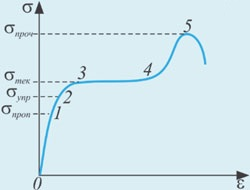
\includegraphics[height=0.35\textwidth]{extra-materials/Диаграмма-растяжения}
		\caption{Диаграмма растяжения}
	\end{figure}
	\textbf{Коэффициент жесткости.}
	\begin{definition}[Коэффициент жесткости]
		Два вида соединений:
		\begin{itemize}
			\item Параллельное соединение. \\
			$k = \frac{ES}{l_0} = \frac{E(\sum_{i = 0} S_i)}{l_0} = \sum_{i = 0} k_i$.
			\item Последовательное соединение. \\
			$\frac{1}{k} = \frac{l_0}{ES} = \frac{\sum_{i = 0} l_{0i}}{ES} = \sum_{i = 0} \frac{1}{k_i}$.
		\end{itemize}
	\end{definition}
	\subsubsection{Гравитация.}
	\begin{definition}
		Исаак Ньютон ($1643 - 1727$ г.). Учился в Кэмбридже. Когда он был на $4$ курсе, произошла эпидемия чумы и он получил бакалавриат без защиты диплома.
	\end{definition}
	\begin{definition}
		Законы Кеплера ($1609 - 1619$):
		\begin{enumerate}
		\item Все планеты движутся по эллипсам, в одном из фокусов которых находится Солнце.
		\item Радиус-вектор планеты за одинаковые промежутки времени заметает равные площади. \\
		\begin{figure}[H]
			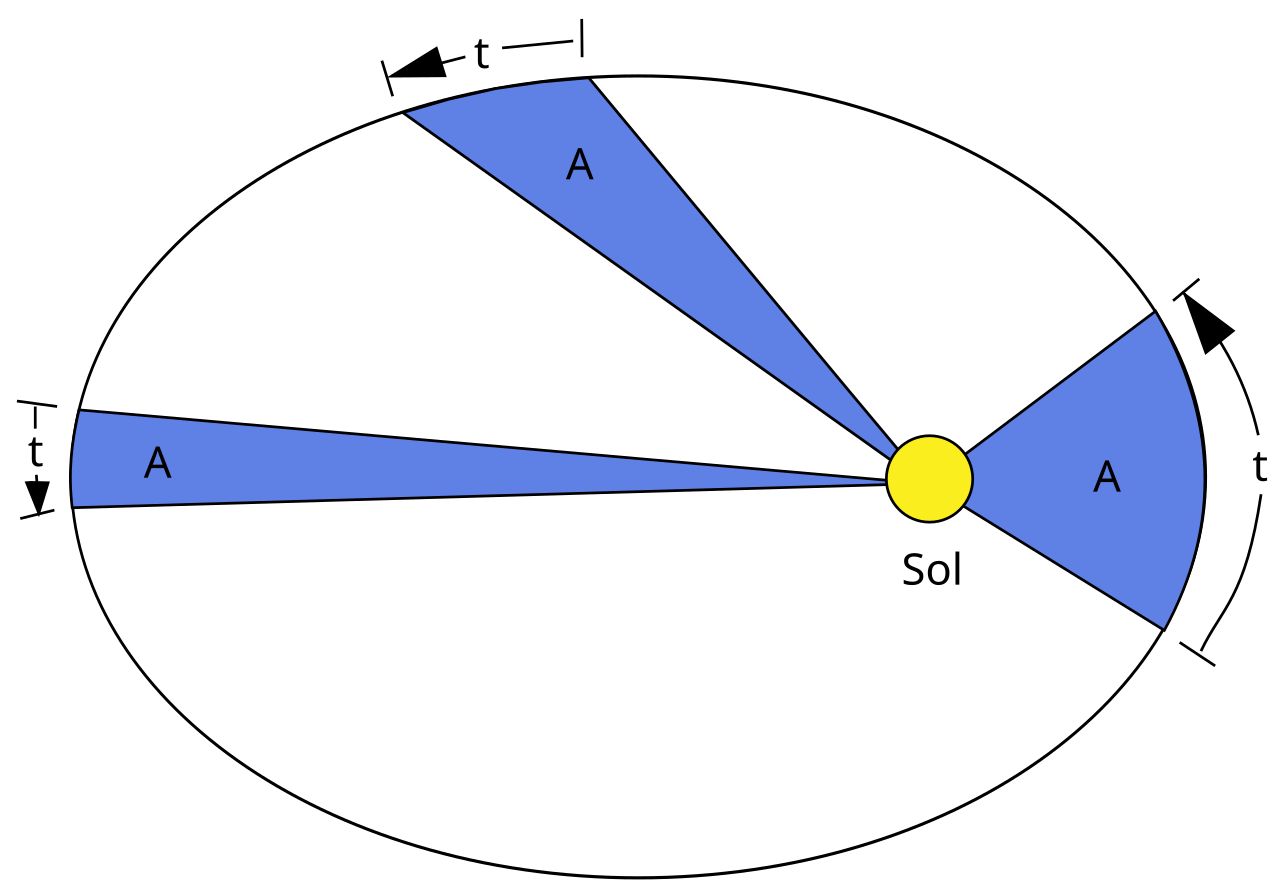
\includegraphics[height=0.25\textwidth]{extra-materials/Второй-закон-Кеплера}
			\caption{Второй закон Кеплера.}
		\end{figure}
		\item $\frac{T_1^2}{T_2^2} = \frac{b_1^3}{b_2^3} = \frac{R_1^3}{R_2^3}$.
		\end{enumerate}
	\end{definition}
	\begin{definition}[Закон всемирного тяготения ($1666$ г.)]
		$F \sim \frac{m_1m_2}{R^2}$. $F_{\text{грав}} = \frac{GM_1M_2}{R^2}$.
	\end{definition}
	\begin{statement}[Границы применения]
		\begin{itemize}
			\item Точечные тела.
			\item Сферические тела, плотность которых зависит только от расстояний до их центров.
		\end{itemize}
	\end{statement}
	\begin{definition}
		Гравитационная масса~--- масса, входящая в закон всемирного тяготения.
	\end{definition}
	\begin{definition}
		Инертная масса~--- масса, входящая во второй закон Ньютона.
	\end{definition}
	\begin{statement}
		Могло быть такое, что они не равны. То, что они равны, стечение обстоятельств в нашей вселенной.
	\end{statement}
	\begin{definition}
		Опыт Кавендиша.
		\begin{figure}[H]
			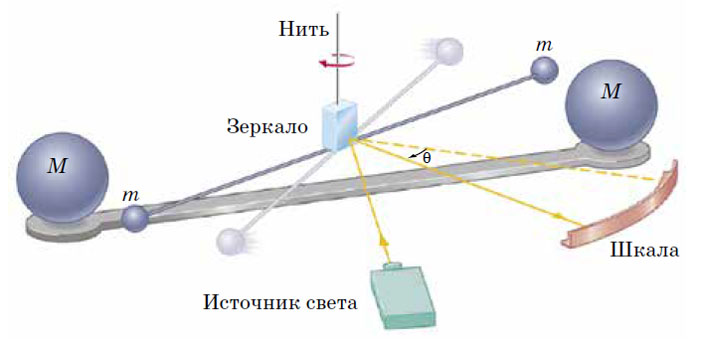
\includegraphics[height=0.25\textwidth]{extra-materials/Опыт-Кавендиша}
			\caption{Опыт Кавендиша*.}
		\end{figure}
		*На самом деле он увеличил точность не с помощью зеркала, а с помощью шкалы Нониуса. $G = 6.67 \cdot 10^{-11} \frac{\text{Н} \cdot \text{м}^2}{\text{кг}^2}$. Но на самом деле он хотел найти $\rho_{\text{земли}} = 5437 \frac{\text{кг}}{\text{м}^3}$. Это очень близко, тк на данный момент принято, что $\rho_{\text{земли}} = 5515 \frac{\text{кг}}{\text{м}^3}$.
	\end{definition}
	\begin{definition}[Ускорение свободного падения]
		$F = G \frac{Mm}{R^2} \rightarrow G \frac{M}{R^2} = g = 9.8$.
	\end{definition}
	\begin{definition}[Первая космическая скорость]
		Это минимальная (для данной высоты над поверхностью планеты) горизонтальная скорость, которую необходимо придать объекту, чтобы он совершал движение по круговой орбите вокруг планеты. \\
		$F_{\text{грав}} = \frac{GMm}{R^2}$; $F_{\text{норм}} = \frac{mv^2}{R}$. \\
		$\frac{GMm}{R^2} = \frac{mv^2}{R}$. \\
		$v = \sqrt{\frac{GM}{R}} = \sqrt{\frac{(6.674 \cdot 10^{-11}) \cdot (5.972 \cdot 10^{24})}{6.371 \cdot 10^6}} \approx 7.91 \cdot 10^3 \frac{\text{м}}{\text{с}}$.
	\end{definition}
	\paragraph{Что видит лунный человечек.} Он всегда вдит землю в одной и той же точке на небе, так как луна вращается вокруг своей оси с такой же скоростью, с какой вращается вокруг земли. Это явление называется "Приливный захват".
	\paragraph{Открытие Нептуна.} В 19 веке ученые заметили, что орбита Урана отклоняется от расчетной, что указывало на влияние неизвестной планеты. Французский математик Урбен Леверье в 1846 году предсказал расположение Нептуна, рассчитав его орбиту на основе этих отклонений. Немецкий астроном Иоганн Галле с помощью телескопа обнаружил Нептун в указанном месте. Нептун стал первой планетой, открытой с помощью математических расчетов, а не прямых наблюдений.
	\begin{figure}[H]
		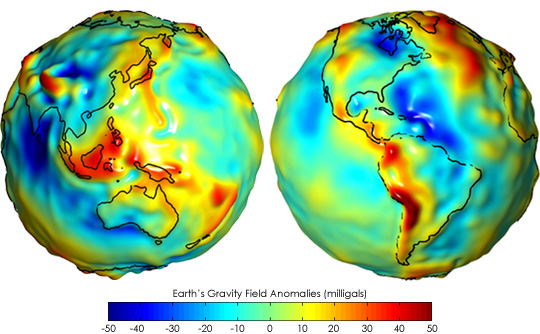
\includegraphics[height=0.25\textwidth]{extra-materials/Геоид}
		\caption{Геоид с увеличенными искажениями и с раскраской, соответствующей гравитационным аномалиям (одна и та же гиря, взвешенная на одних и тех же пружинных весах, будет в «красных местах» тяжелее, а в «синих местах» — легче).}
	\end{figure}
	\subsubsection{Не инерциальные системы отсчета.}
	\begin{definition}[Сила инерции]
		$\vec{F_{\text{и}}} = -m \cdot \vec{a_{\text{пер}}}$. Для нее нет пары, тк на самом деле этой силы не существует.
	\end{definition}
	\subsection{Законы сохранения.}
	\subsubsection{Закон сохранения импульса.}
	\begin{definition}[Импульс]
		$p = m \cdot V; [p] = \frac{\text{кг} \cdot \text{м}}{\text{с}}$.
	\end{definition}
	\begin{definition}[Второй закон Ньютона в импульсной форме]
		$\vec{F} \varDelta t = \varDelta \vec{p} \rightarrow \vec{F} = \frac{\varDelta \vec{p}}{\varDelta t}$.
	\end{definition}
	\begin{definition}[Закон изменения импульса системы]
		$\varDelta \vec{p_{\text{сис}}} = \vec{F_{\text{внеш}}} \cdot \varDelta t$.
	\end{definition}
	\begin{definition}[Закон сохранения импульса]
		Если на систему не действуют внешние силы или их действие скомпенсированно, то импульс системы сохраняется.
	\end{definition}
	\subsection{Реактивное движение.}
	$[\mu] = \frac{\text{кг}}{\text{с}}$~--- скорость расхода топлива, $\vec{u}$~--- скорость топлива в системе отсчета ракеты. \\
	ЗСИ: $M \vec{V} = (M - \mu \varDelta t)(\vec{V} + \varDelta \vec{V}) + \mu \varDelta t (\vec{V} + \vec{u})$. \\
	$0 = M \varDelta \vec{V} - \mu \varDelta t \varDelta \vec{V} + \mu \vec{u} \varDelta t$. \\
	$M \varDelta \vec{V} = -\mu \vec{u} \varDelta t$. \\
	$M \frac{\varDelta \vec{V}}{\varDelta t} = -\mu \vec{u}$. \\
	$M \vec{a} = - \mu \vec{u} = \vec{F_{p}}$. \\
	$\vec{F_{p}} = -\mu \vec{u}$~--- уравнение Мещерского.
	\subsection{Механическая работа.}
	\begin{definition}[Механическая работа]
		$A = Fl \cdot \cos \alpha = (\vec{F}, \vec{l})$. $\alpha$~--- угол между силой и вектором перемещения. $[A] =$ Дж.
	\end{definition}
	\begin{definition}[Мощность]
		$P = \frac{A}{t} = FV \cdot \cos \alpha = (\vec{F}, \vec{V})$. $[P] =$ Вт.
	\end{definition}
	\begin{definition}[Работа силы упругости]
		$A = -\varDelta E_{\text{п}} = -\frac{k (\varDelta x)^2}{2}$.
	\end{definition}
	\subsection{Механическая энергия.}
	\begin{definition}[Кинетическая энергия]
		$E_{\text{к}} = \frac{m \cdot V^2}{2}$. $A = \varDelta E_{\text{к}}$.
	\end{definition}
	\begin{definition}[Потенциальная энергия]
		$E_{\text{п}} = mgh$. $A_{mg} = - \varDelta E_{\text{п}}$.
	\end{definition}
	\begin{definition}[Консервативные силы]
		Силы, работа которых зависит от начального и конечного положения и не зависит от пройденого пути называется консервативными.
	\end{definition}
	\begin{definition}[Закон сохранения энергии]
		$\frac{m \cdot V^2}{2} + mgh = const$. В замкнутой системе, в которой отсутствуют не консервативные силы, энергия сохраняется. Если внешние силы действуют, то изменение механической энергии равно работе внешних сил.
	\end{definition}
	\subsection{Потенциальная энергия силы тяготения.}
	$E_{\text{п}} = \frac{GM_1M_2}{R}$
	\subsection{Статика абсолютно упругого тела.}
	\begin{definition}
		Плечо~--- кратчайшее расстояние от оси вращения тела до линии действия силы.
	\end{definition}
	\begin{definition}
		Момент силы~--- произведение силы на плечо. $M \text{Нм} = F \text{Н} \cdot d \text{м}$.
	\end{definition}
	\begin{definition}
		Условия покоя абсолютно упругого тела:
		\begin{enumerate}
			\item $\sum \vec{F} = 0$
			\item Сумма всех моментов с учетом знака равна $0$ $\Leftrightarrow$ сумма всех моментов, которые вращают по часовой стрелке, равна сумме всех моментов, вращающих по часовой стрелке.
		\end{enumerate}
	\end{definition}
	\begin{definition}[Формула координаты центра масс]
		$x_c = \frac{\sum\limits_i m_i x_i}{m} = \frac{\sum\limits_i m_i x_i}{\sum\limits_i m_i}$. $y_c = \frac{\sum\limits_i m_i y_i}{m} = \frac{\sum\limits_i m_i y_i}{\sum\limits_i m_i}$. $z_c = \frac{\sum\limits_i m_i z_i}{m} = \frac{\sum\limits_i m_i z_i}{\sum\limits_i m_i}$. $\vec{r_c} = \frac{\sum\limits_i m_i \vec{r_i}}{m} = \frac{\sum\limits_i m_i \vec{r_i}}{\sum\limits_i m_i}$.
	\end{definition}
	\begin{definition}
		Виды равновесий.
		\begin{itemize}
			\item Устойчивое~--- положение равновесия, при выводе из которого возникает "возвращающая" сила, которая возвращает его в изначальное положение. Равнодействующая сила возвращает.
			\item Неустойчивое~--- положение равновесия, при выводе из которого тело не возвращается в изначальное положение. Равнодействующая сила не возвращает.
			\item Безразличное~--- равнодействующая сила равна $0$.
		\end{itemize}
	\end{definition}
	\begin{definition}[КПД]
		$\eta = \frac{A_{\text{пол}}}{A_{\text{зат}}} \cdot 100\%$.
	\end{definition}
	\begin{theorem}[О движении центра масс]
		Центр масс тела движется таким образом, как будто он точка массой $m_{\text{общ}}$ и все силы приложены к этой точке.
	\end{theorem}
	\begin{proof}
		$\frac{\varDelta (\varDelta m_i \vec{V}_i)}{\varDelta t} = \frac{\varDelta \vec{p}_i}{\varDelta t} = \sum\limits_{i + k} \vec{F}_{ik} + \sum\limits_i \vec{F}_{\text{внеш}}$ \\
		$\frac{\sum\limits_i \varDelta \varDelta m_i \vec{V}_i}{\varDelta t} = \vec{F}_{\text{внеш}}$ \\
		$\frac{\varDelta \sum\limits_i \varDelta m_i \vec{V}_i}{\varDelta t} = \vec{F}_{\text{внеш}}$ \\
		$r_c' = V_c = \frac{\sum\limits_i \varDelta m_i V_i}{m}$ \\
		$\varDelta \frac{m \vec{V}_c}{\varDelta t} = \vec{F}_{\text{внеш}}$ \\
		$m \vec{a}_c = \vec{F}_{\text{внеш}}$ \\
		$\Rightarrow$ Если внешних сил не действует, то центр масс покоится, если покоился, или движется по инерции, если двигался по инерции.
	\end{proof}
	\subsection{Основное уравнение динамики вращательного движения.}
	\begin{figure}[H]
		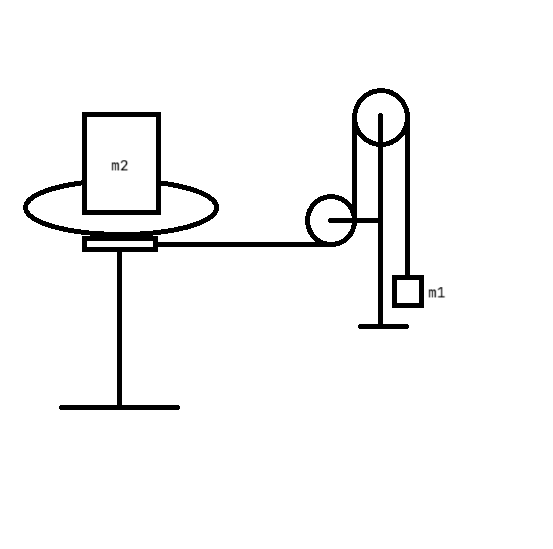
\includegraphics[height=0.5\textwidth]{extra-materials/УравнениеВращательногоДвиженияОпыт}
		\caption{Опыт уравнение вращательного движения.}
	\end{figure}
	Угловое ускорение $\beta$ пропорционально моменту сил $M$.
	\begin{definition}[Момент инерции]
		$I \beta = \sum M$. Для точечного тела $I = mR^2$, для других тел находится интегрированием. $[I] = \text{кг} \cdot \text{м}^2$.
	\end{definition}
	\subsection{Энергия вращательного движения тела.}
	$E = \sum \limits_i \frac{m_iV_i^2}{2} = \sum \limits_i \frac{m_i(\omega \cdot r_i)^2}{2} = \frac{\omega^2}{2} \sum \limits_i m_ir_i^2 = \frac{I\omega^2}{2}$
	\subsection{Теорема Гюйгенса-Штейнера.}
	\begin{theorem}[Гюйгенса-Штейнера]
		Момент инерции $I$ тела относительно произвольной неподвижной точки оси равен сумме момента инерции этого тела $I_c$ относительно параллельной ей оси, проходящей через центр масс тела, и произведения массы тела $m$ на квадрат расстояния $d$ между осями. $I = I_c + md^2$.
	\end{theorem}
	\subsection{Закон сохранения момента импульса.}
	$M = I \beta = I \frac{\omega - \omega_0}{\varDelta t}$ \\
	$M \varDelta t = I \omega - I \omega_0$ \\
	$L = I \omega$~--- момент импульса. $[L] = \frac{\text{кг} \cdot \text{м}^2}{\text{с}}$ \\
	$L = I \omega = m r^2 \frac{V}{r} = p \cdot r$ \\
	$M \varDelta t = \varDelta L$ \\
	$M = \frac{\varDelta L}{\varDelta t} \Rightarrow$ если $M = 0$, то $L = const$.
	\subsection{Колебания.}
	\begin{definition}
		Колебания~--- движения, которые с той или иной точностью повторяющиеся во времени. \\
		Колебания бывают:
		\begin{itemize}
			\item Свободные. Происходят под действием только первоначального запаса энергии. \\
			Условия свободных колебаний:
			\begin{enumerate}
				\item Могут быть только в колебательных системах.
				\item Силы трения малы.
			\end{enumerate}
			\item Вынужденные. Колебания при которых мы помогаем системе колебаться.
			\item Автоколебания. Система, у которой есть собственная энергия, которую она может расходовать на восполнение потраченной энергии.
		\end{itemize}
	\end{definition}
	\begin{definition}
		Величины, характеризующие колебание:
		\begin{quote}
			\begin{definition}
				Период~--- промежуток времени, через который движение повторяется. $T$, $[T] =$ секунды.
			\end{definition}
			\begin{definition}
				Частота~--- обратна величина к периоду, измеряется в Гц, обозначается $\nu$.
			\end{definition}
			\begin{definition}
				максимальное отклонение от положения равновесия. Обозначается $A$/$X_{max}$/$a_{max}$. За период тело проходит $4$ амплитуды.
			\end{definition}
			\begin{definition}
				Фаза колебания~--- где колебания в данный момент, что с ними происходит. Синфазные колебания~--- одинаковые, противофазные~--- разные.
			\end{definition}
		\end{quote}
	\end{definition}
	\begin{definition}
		Гармонические колебания~--- колебания, где возвращающая сила пропорциональна смещению от положения равновесия, взятого с обратным знаком.
	\end{definition}
	\noindent
	График колебательного движения~--- синусоида. \\
	Формула гармонических колебаний. Толкнули: $x = A \sin (\frac{2\pi}{T} t)$; отпустили: $x = A \cos (\frac{2\pi}{T} t)$. \\
	Формула периода для математического маятника: $T = 2\pi\sqrt{\frac{l}{g}}$. \\
	Формула периода для пружинного маятника: $T = 2\pi\sqrt{\frac{m}{k}}$. \\
	\textbf{Резонанс}~--- частота установившихся вынужденных колебаний, равна частоте вынужденной силе.
	\subsection{Механические волны.}
	\textbf{Бегущая волна}~--- возмущение, распространяющееся в пространстве, удаляясь от своего начального положения. \\
	Будем проходить только упругие бегущие волны, в частности~--- звук. \\
	Типы волн:
	\begin{itemize}
		\item \textbf{Продольные}~--- линия колебания совпадает с линией распространения волны. Пример: звук.
		\item \textbf{Поперечные}~--- линия колебания перпендикулярна линии распространения волны.
	\end{itemize}
	\textbf{Длинна волны}~--- расстояние между двумя ближайшими точками, колеблющимися синфазно. Определение номер $2$: расстояние на которое распространилась волна за один период. $\lambda = VT$.
	\subsubsection{Звук.}
	\textbf{Звуковая волна}~--- это передающиеся в пространстве механические колебания молекул вещества (например, воздух). \\
	Человеческое ухо воспринимает частоты от $16$ до $20000$ Гц. Колебания в этом диапазоне называются звуковыми. Мы можем говорить примерно от $50$ до $7000+$ Гц (рекорды). \\
	\textbf{Ультразвук}~--- звуковая волна с частотой больше $20000$ Гц. \\
	\textbf{Инфразвук}~--- звуковая волна с частотой меньше $16$ Гц. \\
	Звуку для распространения нужна среда. В вакууме звука нет. \\
	\textbf{Тембор}~--- совокупность обертонов.
	\subsection{Электромагнитные волны.}
	Цепь из заряженного конденсатора и катушки является колебательной системой и называется простейшим колебательным контуром. \\
	\textbf{Электромагнитная волна}~--- чередование электрического и магнитного поля.
	\subsection{Гидростатика.}
	\textbf{Давление.} $p = \frac{F}{S}$. $\left[p\right] =$ Па. \\
	\textbf{Давление столба жидкости.} $p = \rho g h$. \\
	Давления на все стороны равны. \\
	\textbf{Сила Архимеда.} Суммарная сила действия всех сил давления. $F_{\text{арх}} = \rho_{\text{ж}} g V_{\text{пог}}$.
	\subsection{Гидродинамика.}
	Течение:
	\begin{itemize}
		\item Ламинарное.
		\item Турбулентное (не умем его описывать).
	\end{itemize}
	\textbf{Уравнение неразрывности струи (для несжимаемой жидкости).} $S_1V_1 = S_2V_2$. \\
	\textbf{Закон Бернулли.} $p_1 + \frac{\rho V_1^2}{2} + \rho g h_1 = p_2 + \frac{\rho V_2^2}{2} + \rho g h_2 = const$. \\
	\textbf{Скорость воды с помощью двух сапожков.} $V = \sqrt{\frac{2(p_2 - p_1)}{\rho}}$.
	\subsection{Вязкое трение.}
	$F = \frac{\eta V S}{h}$, $[\eta] = \frac{\text{кг}}{\text{с} \cdot \text{м}}$.
	\section{Молекулярно-кинетическая теория.}
	\begin{definition}
		Точечное тело~--- тело, размерами которого можно пренебречь по сравнению с другими размерами в задаче.
	\end{definition}
	\begin{definition}
		Молекула~--- мельчайшая частица вещества, сохраняющая химические свойства вещества.
	\end{definition}
	\begin{definition}
		Молекулярно-кинетическая теория~--- раздел физики, объясняющий свойства макроскопических тел и тепловых процессов, протекающих в них, на основе представления о том, что тела состоят из отдельных беспорядочно движущихся частиц.
	\end{definition}
	\begin{definition}
		Три основных положения МКТ.
		\begin{itemize}
			\item Все вещества состоят из молекул и атомов.
			\item Эти частицы находятся в непрерывно хаотичном движении.
			\item Между молекулами и атомами существуют силы притяжения и отталкивания.
		\end{itemize}
	\end{definition}
	\subsection{Тепловые явления.}
	\begin{definition}
		Тепловые явления~--- явления, которые связанные с изменениями температуры.
	\end{definition}
	\begin{definition}
		Тепловое движение~--- беспорядочное движение молекул.
	\end{definition}
	\begin{definition}
		Термодинамика~--- теория тепловых явлений, в которых не учитывается молекулярное строение тел.
	\end{definition}
	\begin{definition}[Масса частиц]
		Относительная молекулярная масса: $M_r = \frac{m_0}{\frac{1}{12} m_{0C}} = \text{аем}$.
	\end{definition}
	\begin{definition}
		Один моль ($\nu$)~--- количество вещества в котором содержится столько же молекул или атомов, сколько атомов содержится в углероде массой $12$ г.
	\end{definition}
	\begin{definition}[Число Авогадро]
		Количество атомов в одном моле вещества. $N_a = 6.02 \cdot 10^{23} \text{ моль}^{-1}$. $\nu = \frac{N}{N_a}$.
	\end{definition}
	\begin{definition}
		Молярная масса~--- масса одного моля вещества.
	\end{definition}
	\subsection{Идеальный газ. Основное уравнение МКТ.}
	\begin{definition}
		Идеальный газ~--- газ, взаимодействием молекул которого можно пренебречь.
		\begin{itemize}
			\item Суммарный объем всех молекул пренебрежимо мало по сравнению с объемом сосуда.
			\item Удары об сосуд абсолютно упругие, без диффузии.
			\item Время удара много меньше времени свободного пробега.
			\item Нет дальнодействующего взаимодействия.
		\end{itemize}
	\end{definition}
	\begin{definition}[Основное уравнение МКТ.]
		$p = \dfrac{1}{3} m_0 n \overline{\mathcal{V}^2}$.
	\end{definition}
	\begin{corollary}
		$p = \dfrac{2}{3} n \overline{E}$.
	\end{corollary}
	\subsection{Температура.}
	\begin{statement}
		$\overline{E} = \dfrac{3}{2}KT$.
	\end{statement}
	\begin{statement}
		$\overline{\mathcal{V}^2} = \dfrac{3KT}{m}$.
	\end{statement}
	\subsection{Уравнение Менделеева-Клапейрон. Изопроцессы}
	$p = nKT = \dfrac{N}{V}KT = \dfrac{N_a \nu KT}{V}$. $N_a \cdot K = 6.02 \cdot 10^{23} \dfrac{1}{\text{моль}} \cdot 1.38 \cdot 10^{-23} \dfrac{\text{Дж}}{\text{К}} \Leftrightarrow R = 8.31 \dfrac{\text{Дж}}{\text{моль} \cdot \text{К}}$~--- универсальная газовая постоянная. \\
	\begin{definition}[Уравнение Менделеева-Клапейрон]
		$pV = \nu RT$.
	\end{definition}
	\begin{xltabular}{\textwidth}{|X|X|X|X|X|}
		\hline
		Изопроцесс & Const & Закон & График & Комментарий \\
		\hline
		Изотермический & $T$ & $p_1V_1 = p_2V_2$; Закон Бойля-Мариотта & Гипербола ($P$ от $V$); Вертикальная палка ($P$ от $T$); Вертикальная палка ($V$ от $T$) & \\
		\hline
		Изохорный & $V$ & $\dfrac{p_1}{T_1} = \dfrac{p_2}{T_2}$; Закон Шарля & Вертикальная палка ($P$ от $V$); Прямая ($P$ от $T$); Горизонтальная палка ($V$ от $T$) & \\
		\hline
		Изобарный & $p$ & $\dfrac{V_1}{T_1} = \dfrac{V_2}{T_2}$ & Горизонтальная палка ($P$ от $V$); Горизонтальная палка ($P$ от $T$); Прямая ($V$ от $T$) & \\
		\hline
	\end{xltabular}
\end{document}
